\documentclass[10pt]{scrartcl}
\usepackage[mdthm,colorsec,noauthor,noasy]{evan}
\usepackage{handout}
\usepackage[T1]{fontenc}
\usepackage{lmodern}
\usepackage{listings}
\lstset{language=Python,emptylines=1,basicstyle=\ttfamily\normalsize,identifierstyle=\color{black},keywordstyle=\color{NavyBlue},commentstyle=\color{black!60},stringstyle=\color{RawSienna},showstringspaces=false,columns=fullflexible,keepspaces=true,upquote=true,aboveskip=5pt,belowskip=5pt}
\newcommand{\py}[1]{\texttt{#1}}
\newcommand{\hint}[1]{\par\emph{Hint:} #1\par}
\newcommand{\codeblock}[1]{\par\noindent\begin{minipage}{\linewidth}\csname code#1\endcsname\end{minipage}\par}
\expandafter\def\csname codeteamwork\endcsname{\lstinputlisting[firstline=4,lastline=13]{discussion_solutions.py}}
\expandafter\def\csname codekeeper\endcsname{\lstinputlisting[firstline=17,lastline=24]{discussion_solutions.py}}
\expandafter\def\csname codefind_digit\endcsname{\lstinputlisting[firstline=28,lastline=30]{discussion_solutions.py}}
\expandafter\def\csname codematch_k\endcsname{\lstinputlisting[firstline=34,lastline=41]{discussion_solutions.py}}
\expandafter\def\csname codewhich\endcsname{\lstinputlisting[firstline=45,lastline=53]{discussion_solutions.py}}
\expandafter\def\csname codeevery\endcsname{\lstinputlisting[firstline=57,lastline=65]{discussion_solutions.py}}
\expandafter\def\csname codecount_if\endcsname{\lstinputlisting[firstline=69,lastline=80]{discussion_solutions.py}}
\expandafter\def\csname codenew_print\endcsname{\lstinputlisting[firstline=4,lastline=10]{exam_solutions.py}}
\expandafter\def\csname codegap_tool\endcsname{\lstinputlisting[firstline=14,lastline=19]{exam_solutions.py}}
\expandafter\def\csname codemake_gap\endcsname{\lstinputlisting[firstline=23,lastline=35]{exam_solutions.py}}
\expandafter\def\csname codefunsquare\endcsname{\lstinputlisting[firstline=39,lastline=59]{exam_solutions.py}}
\expandafter\def\csname codesummation\endcsname{\lstinputlisting[firstline=4,lastline=9]{examples.py}}
\expandafter\def\csname codetwice\endcsname{\lstinputlisting[firstline=13,lastline=19]{examples.py}}
\expandafter\def\csname coderetained\endcsname{\lstinputlisting[firstline=23,lastline=32]{examples.py}}
\expandafter\def\csname codecurry\endcsname{\lstinputlisting[firstline=36,lastline=41]{examples.py}}
\expandafter\def\csname codenearest\endcsname{\lstinputlisting[firstline=56,lastline=64]{examples.py}}
\expandafter\def\csname codepiecewise\endcsname{\lstinputlisting[firstline=4,lastline=7]{lab_solutions.py}}
\expandafter\def\csname codecount_cond\endcsname{\lstinputlisting[firstline=11,lastline=19]{lab_solutions.py}}
\expandafter\def\csname codecycle\endcsname{\lstinputlisting[firstline=23,lastline=37]{lab_solutions.py}}
\expandafter\def\csname codelab_diagram\endcsname{\lstinputlisting[firstline=41,lastline=57]{lab_solutions.py}}

\title{CS 61A --- Week 3}
\subtitle{Solutions: Lab 2, Discussion 2 and actual exam practice}
\author{}\date{}\ihead{}
\begin{document}\maketitle
\begin{prob}
\textbf{Lab 2 Q1: The Truth Will Prevail.} \idea{Identify the last operand actually evaluated; record its value separately from its output effect.}
\begin{center}\begin{tabular}{l|l}
expression&prompt display\\\hline
\py{True and 13}&\py{13}\\
\py{False or 0}&\py{0}\\
\py{not 10}&\py{False}\\
\py{not None}&\py{True}\\
\py{True and 1/0}&\py{ZeroDivisionError} (ERROR)\\
\py{True or 1/0}&\py{True}\\
\py{-1 and 1 > 0}&\py{True}\\
\py{-1 or 5}&\py{-1}\\
\py{(1+1) and 1}&\py{1}\\
\py{print(3) or ''}&\py{3}, then \py{''}\\
\py{0 or f(1)}&\py{'positive'}\\
\py{f(0) or f(-1)}&\py{'zero'}\\
\py{f(0) and f(-1)}&\py{''}
\end{tabular}\end{center}
\begin{steps}
\ii The true left operand of \py{True and 1/0} requires evaluating the division; the true left operand of \py{True or 1/0} skips it. A negative number is true, so \py{-1 and (1>0)} reaches the comparison.
\ii \py{print(3)} prints 3 and returns false-valued None. The or expression therefore returns the empty string, which appears as \py{''} at the prompt.
\ii \py{f(0)} returns nonempty \py{'zero'}, so or stops there but and continues to \py{f(-1)}, which returns the empty string.
\end{steps}
\end{prob}
\begin{prob}
\textbf{Lab 2 Q2: Higher-Order Functions.} \idea{Keep the returned pie function distinct from the string it returns when called.}
\begin{center}\begin{tabular}{l|l}
input&display\\\hline
\py{chocolate=cake()}&\py{beets}\\
\py{chocolate}&FUNCTION (pie)\\
\py{chocolate()}&\py{sweets}, then \py{'cake'}\\
\py{more\_chocolate,more\_cake=chocolate(),cake}&\py{sweets}\\
\py{more\_chocolate}&\py{'cake'}\\
\py{snake(10,20)} before rebinding cake&FUNCTION (pie)\\
\py{snake(10,20)()} before rebinding cake&\py{sweets}, then \py{'cake'}\\
\py{snake(10,20)} after \py{cake='cake'}&\py{30}
\end{tabular}\end{center}
\begin{steps}
\ii Calling cake prints beets and returns pie; merely referring to chocolate does not call pie. Calling chocolate prints sweets and returns a string.
\ii Simultaneous assignment computes both old right-hand values first. more\_chocolate receives the string; more\_cake receives the original cake function. No returned string is displayed by the assignment itself.
\ii Initially cake and more\_cake refer to the same function, so snake returns chocolate. After cake is rebound to a string they differ, so snake instead returns 10+20.
\end{steps}
\end{prob}
\begin{prob}
\textbf{Lab 2 Q3: Lambda.} \idea{A function is created before its body is evaluated; the body runs only after the corresponding call.}
\begin{center}\begin{tabular}{l|l}
input&display\\\hline
\py{lambda x:x}&FUNCTION\\
\py{a(5)}&\py{5}\\
\py{(lambda:3)()}&\py{3}\\
\py{c}&FUNCTION (zero-argument returned lambda)\\
\py{c()}&\py{12}\\
\py{d(square)}&\py{16}\\
\py{higher\_order\_lambda(g)(2)}&\py{4}\\
\py{call\_thrice(lambda y:y+2)(5)}&\py{11}\\
\py{print\_lambda}&FUNCTION\\
\py{one\_thousand=print\_lambda(1000)}&\py{1000}\\
\py{print(one\_thousand)}&\py{None}
\end{tabular}\end{center}
\begin{steps}
\ii \py{b(8,4)} returns a zero-argument function retaining x = 8 and y = 4. Its later call computes 12. \py{d(square)} calls square on 4 and returns 16.
\ii The higher-order lambda calls the supplied g on 2; call\_thrice applies the increment-by 2 three times: $5\to7\to9\to11$.
\ii print\_lambda returns None after its output effect. The assignment stores None; printing that value displays the word None. The assignment and all other definitions produce no additional prompt display.
\end{steps}
\end{prob}
\begin{prob}
\textbf{Lab 2 Q4: Piecewise.} \idea{Wait for x before choosing which retained function to apply.}
\codeblock{piecewise}
\begin{steps}
\ii The function h retains access to f,g,b. A call to piecewise itself calls neither branch function.
\ii With b = 0, negate and identity, h(6) chooses identity and gives 6; h $(-1)$ chooses negate and gives 1. At x=b the g branch is selected.
\end{steps}
\end{prob}
\begin{prob}
\textbf{Lab 2 Q5: Count Cond.} \idea{Retain the predicate, then start a new index and counter whenever the returned function receives n.}
\codeblock{count_cond}
\begin{steps}
\ii Before each test, total counts the successful indices 1 through $i-1$. Testing condition(n,i) and then advancing i preserves this statement. At i=n+1 every permitted index has been tested.
\ii \py{count\_cond(lambda n,i:sum\_digits(n*i)==5)} gives 1 at 10 (50), and 4 at 50 (50,500,1400,2300). Each listed product has digit sum 5.
\ii \py{count\_cond(lambda n,i:is\_prime(i))} gives 1,2,2,3,8 at 2,3,4,5,20. The primes up to 20 are 2,3,5,7,11,13,17,19. Use the lab's supplied helpers; the positive-only primality helper is called only on i $\ge1$.
\end{steps}
\end{prob}
\begin{prob}
\textbf{Lab 2 Q6: HOF Diagram Practice.} \idea{The original f and the later f are different function values. Resolve the right-hand call before replacing its global name.}
\begin{steps}
\ii The second definition replaces the first global f. Evaluating \py{f(g,n)} calls that new f with its local parameter f bound to the original g function, and local x = 7. It reads global n = 7, then calls g(14).
\ii g(14) has local x = 14,n = 9 and creates h with this call as parent. It returns h. The outer f also returns h, which becomes the new global f.
\ii The global lambda receives h as y and calls y(). h finds x = 14 in its parent and returns 15. The lambda returns 15, then the assignment rebinds global g to 15. Global n stays 7.
\end{steps}
\begin{fig}
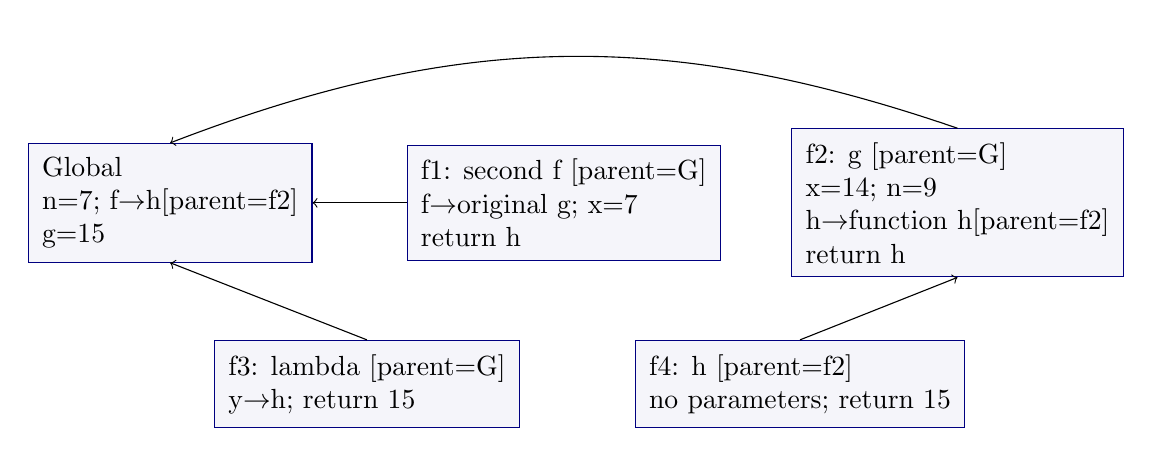
\begin{tikzpicture}[box/.style={draw=NavyBlue,fill=NavyBlue!4,align=left,inner sep=5pt},every node/.style={font=\normalsize}]
\node[box] (G) at (0,0) {Global\\n=7; f$\to$h[parent=f2]\\g=15};
\node[box] (a) at (5,0) {f1: second f [parent=G]\\f$\to$original g; x=7\\return h};
\node[box] (b) at (10,0) {f2: g [parent=G]\\x=14; n=9\\h$\to$function h[parent=f2]\\return h};
\node[box] (c) at (2.5,-2.3) {f3: lambda [parent=G]\\y$\to$h; return 15};
\node[box] (d) at (8,-2.3) {f4: h [parent=f2]\\no parameters; return 15};
\draw[->] (a.west)--(G.east);
\draw[->] (b.north) to[bend right=20] (G.north);
\draw[->] (c.north)--(G.south);
\draw[->] (d.north)--(b.south);
\end{tikzpicture}
\figcap{Arrows are parent links, not call order. Global f and f2's h refer to the same returned function; original global g is replaced only after the lambda finishes.}
\end{fig}
The first f(x), with its unused local n = 8, is never called. Its name was replaced by the second definition; therefore it creates no call frame. The four actual user-defined calls are f, g, lambda, h.
\end{prob}
\begin{prob}
\textbf{Lab 2 Q7: Week 3 Survey.} \idea{A completion token comes from the actual survey; it is not a programming exercise with a deducible answer.}
\begin{steps}
\ii The linked form says it no longer accepts responses. Its question text and completion token are unavailable here.
\ii The starter's hash check checks a supplied token; it does not supply the token. No invented passphrase or personal responses are included.
\end{steps}
\end{prob}
\begin{prob}
\textbf{Lab 2 Q8 (optional): Cycle.} \idea{The counter tells both how many functions have run and which of the three must run next.}
\codeblock{cycle}
\begin{steps}
\ii f1,f2,f3 are retained by g; n is retained by h. On each call of h, i starts 0 and x is that call's input.
\ii After i iterations, x is the result of the first i cyclic applications. Remainders 0,1,2 select f1,f2,f3; increasing i preserves the statement.
\ii For input 2, add1/times2/add3 give $2\to3\to6\to9\to10$ through four steps. At six steps on 1, $1\to2\to4\to7\to8\to16\to19$. At n = 0 the loop skips all functions and returns the original input 5.
\end{steps}
\end{prob}

\section{Discussion 2}
\begin{prob}
\textbf{Q1: Warm Up.} \idea{Use a separate local x for each lambda call.}
\begin{steps}
\ii The outer call binds x = 5. The inner call binds its own x = 4 but its body is the constant 3.
\ii The outer body is therefore $2\cdot3\cdot5=30$. Assignment binds result 30 and produces no prompt output.
\end{steps}
\end{prob}
\begin{prob}
\textbf{Q2: Teamwork.} \idea{Determine the global t used by team before considering dream's separate local t.}
\begin{steps}
\ii The right side calls dream with work bound to the original team function and s = 4. Its condition calls that team on 2.
\ii team(2) reads global t=abs and returns abs(2)$-1=1$. This is true, so dream assigns its own local t=not 4=False, then returns \py{not False}, which is \py{True}.
\ii The final and therefore evaluates global t=abs and returns it. Only then does assignment change global team to abs; global work = 3 and t=abs remain unchanged.
\end{steps}
\begin{fig}
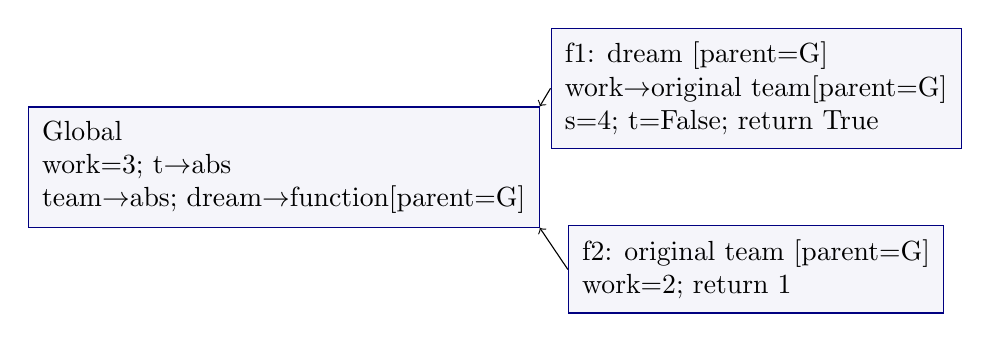
\begin{tikzpicture}[box/.style={draw=NavyBlue,fill=NavyBlue!4,align=left,inner sep=5pt}]
\node[box] (g) at (0,0) {Global\\work=3; t$\to$abs\\team$\to$abs; dream$\to$function[parent=G]};
\node[box] (d) at (6,1) {f1: dream [parent=G]\\work$\to$original team[parent=G]\\s=4; t=False; return True};
\node[box] (t) at (6,-1.3) {f2: original team [parent=G]\\work=2; return 1};
\draw[->] (d.west)--(g.north east);\draw[->] (t.west)--(g.south east);
\end{tikzpicture}
\figcap{Both call frames have Global as parent. The team call finds global abs, not the dream call's local t.}
\end{fig}
\end{prob}
\begin{prob}
\textbf{Q3: Make Keeper.} \idea{Retain n, then scan its finite interval with the predicate supplied later.}
\codeblock{keeper}
\begin{steps}
\ii Before each test all matching values below i have been printed once in increasing order. Test i, print it only if cond says true, and increase i.
\ii At i=n+1 every permitted value has been considered. For n = 5 an even predicate prints 2,4; true prints 1,2,3,4,5; false prints nothing. With no explicit return, each returned-function call returns None.
\end{steps}
\end{prob}
\begin{prob}
\textbf{Q4: Digit Finder.} \idea{Keep the requested position k while waiting for the integer x.}
\codeblock{find_digit}
\begin{steps}
\ii For k = 2,x = 3456, division by 10 leaves 345; remainder 10 gives 5. For 5678 it leaves 567 and gives 7.
\ii At k = 1,x = 10, no digits are removed and remainder 10 is 0. For k = 4,x = 789, division by 1000 is 0, so the absent digit gives 0. The displayed implementation uses no string or indexing operation.
\end{steps}
\end{prob}
\begin{prob}
\textbf{Q5: Match Maker.} \idea{One unequal existing pair disproves the claim; success requires all such pairs to pass.}
\codeblock{match_k}
\begin{steps}
\ii Compare the last digit with the last digit after stripping k places. After stripping one more digit from x, the next adjacent position is ready; no pair is omitted.
\ii For 1010,k = 2, compare 0 with 0, then 1 with 1. For 2010,k = 2, the second comparison is 1 with 2, so return false. For 123123,k = 3 all three corresponding pairs agree; at k = 2 the first pair is 3 versus 1 and fails.
\ii When x has at most k digits the condition is false, since no full pair remains. Thus the single digit 1 at k = 1 returns true. For 2111111111111111 the scan eventually reaches 21 and detects 1 versus 2.
\end{steps}
\end{prob}
\begin{prob}
\textbf{Q6 (optional): Which One.} \idea{The first return in each call makes the later statements unreachable.}
\begin{steps}
\ii which binds local one = 3 and creates this with that frame as parent. It returns this before the assignment one = 4.
\ii The returned this finds one = 3 in that parent and returns it before its second return. Thus \py{which()()} displays 3; global one remains 1.
\end{steps}
\begin{fig}
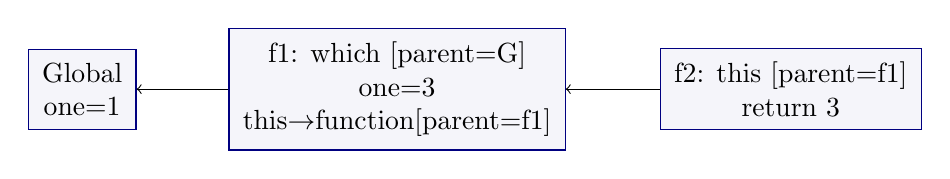
\begin{tikzpicture}[box/.style={draw=NavyBlue,fill=NavyBlue!4,align=center,inner sep=5pt}]
\node[box] (g) at (0,0) {Global\\one=1};
\node[box] (w) at (4,0) {f1: which [parent=G]\\one=3\\this$\to$function[parent=f1]};
\node[box] (t) at (9,0) {f2: this [parent=f1]\\return 3};
\draw[->] (t.west)--(w.east);\draw[->] (w.west)--(g.east);
\end{tikzpicture}
\figcap{The first matching binding on the parent chain is local one = 3. Global one = 1 is not used.}
\end{fig}
\end{prob}
\begin{prob}
\textbf{Q7 (optional): Choose Wisely.} \idea{Reject the first failing digit; if there is no failure before the end, every digit passed.}
\codeblock{every}
\begin{steps}
\ii The blanks are \py{not t(n\%10)}, \py{return False}, \py{True}, and \py{digit}. Before each test all removed digits passed t.
\ii For 37511 the odd-digit tests on 1,1,5,7,3 all pass. For 2023, the first 3 passes but the next 2 fails, so the result is false.
\end{steps}
\end{prob}
\begin{prob}
\textbf{Q8 (optional): Nice Dice.} \idea{Count passing digits once, then supply the threshold as a new predicate.}
\codeblock{count_if}
\begin{steps}
\ii The first blank is \py{f(n\%10)}. Before each test, count is the number of removed digits passing f. Testing the last digit, incrementing if necessary and removing it preserves the statement.
\ii The second blank is \py{lambda d:d>=k}. It retains k and lets count\_if perform the entire scan; no second loop is needed.
\ii In 431663334231 there are five 3s, so the equality test counts 5. The only digits below 3 are 1,2,1; the other 9 meet threshold 3.
\end{steps}
\end{prob}

\section{Actual exam practice}
\begin{prob}
\textbf{Fall 2022 MT 1Q4(a): Funsquare.} \idea{Check the outer interface and the deferred inner computation separately.}
\begin{steps}
\ii D and F are correct: each accepts only f and returns a one-argument function whose later body computes f(f(x)). For triple at 5 the inner call gives 15, then the outer gives 45.
\ii A immediately calls f on the function f, which is not the requested later input. B returns a zero-argument function, which cannot accept x and also has the wrong body f(f).
\ii C and E each require an additional outer x, so funsquare(triple) raises TypeError. C's inner computation would be suitable after two outer arguments, but that is the wrong required signature; E directly returns a result rather than the required function.
\end{steps}
\end{prob}
\begin{prob}
\textbf{Fall 2026 MT 1Q2: New Print.} \idea{Name each wrapper separately; its parameter named print still refers to the previous wrapper after the global name is rebound.}
\begin{steps}
\ii Let P0 be built-in print. The first returned f is P1, whose parent retains print=P0. The second returned f is P2, whose different parent retains print=P1. Global og=P0, print=P2.
\ii Calling P2(2) first calls P1(2). P1 calls P0(2), printing 2 and receiving None, so P1 returns 2. P2 therefore has value 2 and enters its if.
\ii P2 returns P1('What?'). That calls P0('What?'), printing What? and returning None, so P1 returns the string 'What?'. Finally og prints the words print returned followed by that returned string.
\end{steps}
\begin{fig}
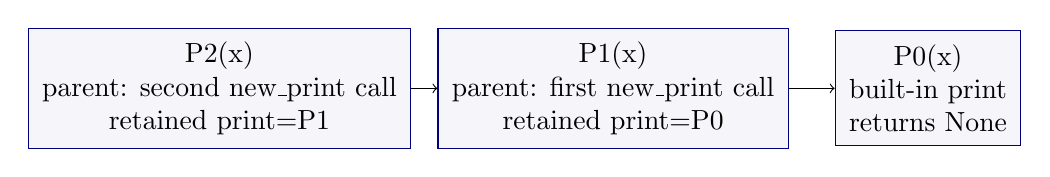
\begin{tikzpicture}[box/.style={draw=NavyBlue,fill=NavyBlue!4,align=center,inner sep=5pt}]
\node[box] (p2) at (0,0) {P2(x)\\parent: second new\_print call\\retained print=P1};
\node[box] (p1) at (5,0) {P1(x)\\parent: first new\_print call\\retained print=P0};
\node[box] (p0) at (9,0) {P0(x)\\built-in print\\returns None};
\draw[->] (p2.east)--(p1.west);\draw[->] (p1.east)--(p0.west);
\end{tikzpicture}
\figcap{Each wrapper calls the print stored in its own parent. Rebinding the global name does not make P1 call P2.}
\end{fig}
The complete output is:
\begin{verbatim}
2
What?
print returned What?
\end{verbatim}
\end{prob}
\begin{prob}
\textbf{Fall 2026 MT 1Q4.3: Make Gap (optional A+).} \idea{Gap needs a consecutive index 1,2,\ldots. Count how many indices pass use, then translate its jth index to the jth passing original index.}
\codeblock{make_gap}
\begin{steps}
\ii In the supplied f, i is the number of indices tested and y the number passing use. For \py{go=lambda y,i:i<n}, the loop tests exactly 1 through n; \py{then=lambda y,i:y} returns their passing count m.
\ii For any 1 $\le j\le m$, \py{go=lambda y,i:y<j} stops at the jth passing index. Returning i locates that index. Applying term there supplies the jth value of the selected sequence to gap.
\ii For a stable predicate use, gap therefore compares exactly consecutive selected values. With odd indices through 8, the first f returns 4; the inner f calls locate 1,3,5,7, whose mod 5 values are 1,3,0,2. Differences 2,3,2 have maximum 3.
\ii At least two indices pass, so gap's sequence has at least two terms and every requested jth index exists. The answer uses only the permitted lambdas and calls. The if inside supplied f is provided code, not a forbidden if introduced in the answer.
\end{steps}
\end{prob}
\end{document}
